\documentclass{beamer}
\usepackage{ctex}
\usepackage[export]{adjustbox}
\usepackage{listings}
\usepackage{xcolor}

\usetheme{focus}

\definecolor{codegreen}{RGB}{50 200 50}
\definecolor{codeblue}{RGB}{50 50 200}
\definecolor{codered}{RGB}{200 50 50}
\tikzset{
    global scale/.style={scale=#1,every node/.append style={scale=#1}},
    CC1/.style ={circle,minimum width = 30pt, minimum height =30pt, draw=black},
    CC2/.style ={circle,minimum width = 30pt, minimum height =30pt, draw=black, fill=blue!20},
    RA1/.style ={rectangle,minimum width = 30pt, minimum height =20pt, draw=black},
    RA2/.style ={rectangle,minimum width = 1cm, minimum height = 1cm, draw=black}
}

\title{算法分析与设计II}
\subtitle{2022-2023-2}
\date{Last Modified: 2023.1.16}
\institute{\vspace{2em} 数学与计算机学院 \\ 数据科学与大数据技术}
\titlegraphic{\vspace{5em} 
\includegraphics[scale=0.3]{fig/jlnu.pdf}}

\lstset{
    columns=flexible,       
    numbers=left,  
    numberstyle=\footnotesize\color{darkgray},  
    frame=shadowbox, 
    rulesepcolor= \color{gray}, 
    keywordstyle=\color{codeblue},         
    commentstyle=\color{codegreen},  
    stringstyle=\color{codered}, 
    showstringspaces=false,  
    xleftmargin=3em,
    xrightmargin=1em,              
    language=c++                           
}

\tikzset{
    CC1/.style ={
    circle,
    minimum width = 30pt, 
    minimum height =30pt, 
    draw=black
    }
}

\begin{document}
\frame{\titlepage}
\section{4. 动态规划}
\begin{frame}{4.1 基础动态规划问题}
    \begin{enumerate}
        \item 动态规划的一个特征是问题有\textcolor{blue}{重叠的子问题},与分治算法类似,可以将原问题分解为子问题,使用相同的规则进行求解
        \vfill
        \item 动态规划的另一个重要特征是\textcolor{blue}{最优子结构}(Optimal substructure) ,依据的是贝尔曼最优化原理(Bellman's principle of optimality) : 作为整个过程的最优策略具有这样的性质,无论过去的状态和决策如何,对先前决策所形成的状态而言,余下的诸决策必构成最优策略
    \end{enumerate}
    \vfill
    \begin{itemize}
        \item 以上两点也是判断一个问题是否适用动态规划的主要依据
    \end{itemize}
\end{frame}
\begin{frame}{解最短路问题}
    \begin{columns}
        \column{0.65\textwidth}
        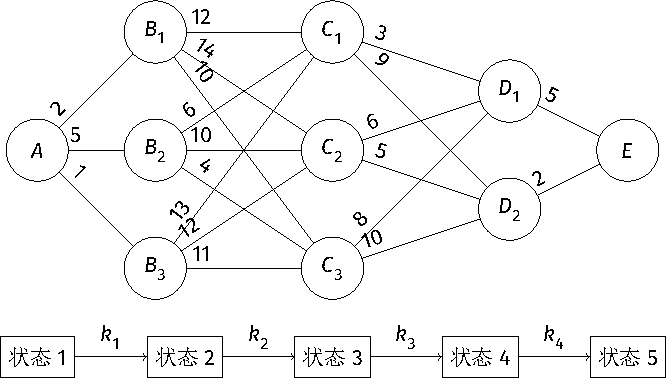
\includegraphics[scale=.65]{fig/4-1.pdf}
        \column{0.35\textwidth}
            \begin{enumerate}[(1)]
                \scriptsize{\item 阶段(stage): $k$}
                \pause
                \item 状态(state): $s_k$
            \end{enumerate}
            \begin{table}
                \scriptsize{
                \begin{tabular}{c|l}
                \hline
                阶段1 & $s_1=[A]$ \\\hline
                阶段2 & $s_2=[B_1,B_2,B_3]$ \\\hline
                阶段3 & $s_3=[C_1,C_2,C_3]$ \\\hline
                阶段4 & $s_4=[D_1,D_2]$ \\\hline
                阶段5 & $s_5=[E]$ \\\hline
                \end{tabular}
                }
            \end{table}
            \pause
            \begin{enumerate}[(3)]
                \scriptsize{\item 决策(decision)}
            \end{enumerate}
            \begin{itemize}
                \scriptsize{\item 决策变量$x_k(s_k)$表示第$k$阶段状态为$s_k$时对方案的选择. $D_k(s_k)$表示$k$阶段状态为$s_k$时决策允许的取值集合}
                \item $D_2(B_1)=[C_1,C_2,C_3]$
            \end{itemize}
    \end{columns}
\end{frame}
\begin{frame}{解最短路问题}
    \begin{columns}
        \column{0.65\textwidth}
        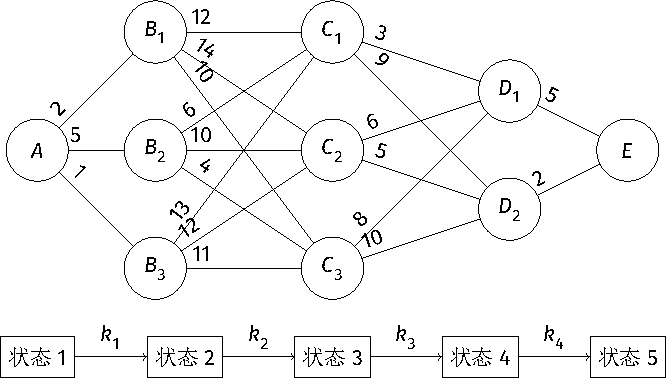
\includegraphics[scale=.65]{fig/4-1.pdf}
        \column{0.35\textwidth}
            \begin{enumerate}[(4)]
                \scriptsize{\item 策略(policy)和子策略(subpolicy)}
            \end{enumerate}
            \begin{itemize}
                \scriptsize{\item 动态规划问题各阶段决策组成的序列总体称为一个策略}
                \item $[x_1(s_1),x_2(s_2),...,x_n(s_n)]$是$n$阶段DP一个策略
            \end{itemize}
            \pause
            \begin{enumerate}[(5)]
                \scriptsize{\item 状态转移}
            \end{enumerate}
            \begin{itemize}
                \scriptsize{\item 从$s_k$的某一状态值出发,当决策变量$x_k(s_k)$的取值决定后,下一阶段状态变量$s_{k+1}$的取值也随之确定.这种从上一阶段的某一状态到下一阶段某一状态称为状态转移}
                \item $s_{k+1}=T(s_k,x_k(s_k))$
                \item 或 $s_{k+1}=T(s_k,x_k)$
            \end{itemize}
    \end{columns}
\end{frame}
\begin{frame}{解最短路问题}
    \begin{columns}
        \column{0.65\textwidth}
        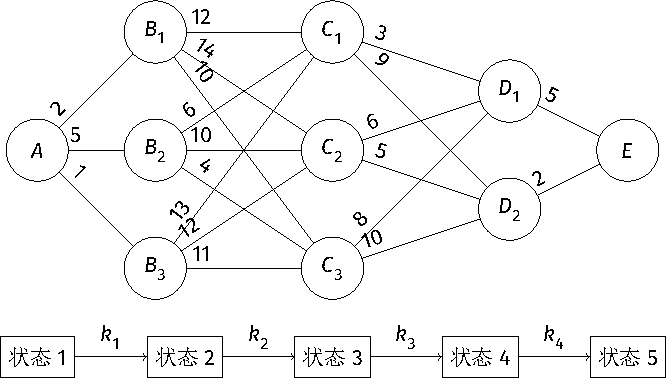
\includegraphics[scale=.65]{fig/4-1.pdf}
        \column{0.35\textwidth}
            \begin{enumerate}[(6)]
                \scriptsize{\item 目标函数}
            \end{enumerate}
            \begin{itemize}
                \scriptsize{\item 目标函数是用来衡量实现过程优劣的一种数量指标.它是从状态$s_k$出发至过程最终,当采取某种策略时,按预定标准得到的效益值}
                \item $V_{k,n}(s_k,x_k,s_{k+1},x_{k+1},...,s_n)$
            \end{itemize}
            \pause
            \begin{enumerate}[(7)]
                \scriptsize{\item 最优目标函数}
            \end{enumerate}
            \begin{itemize}
                \scriptsize{\item 对某一确定状态选取最优策略后得到的指标函数值,也就是对应某一最优子策略的某种效益度量}
                \item $f_k(s_k)=optV_{k,n}$
            \end{itemize}
    \end{columns}
\end{frame}
\begin{frame}
    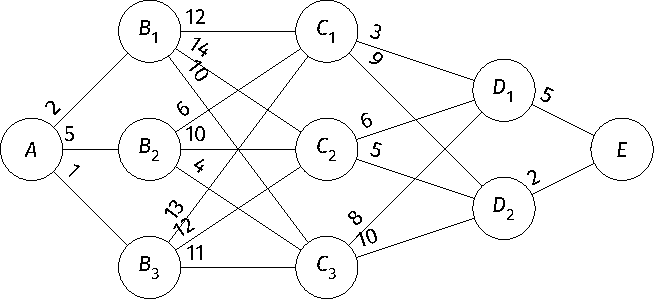
\includegraphics{fig/4-2-1.pdf}
    \vfill
    $$f_k(s_k)=\min \limits_{x_k\in D_k(s_k),k=4,3,2,1} [d_k(s_k,x_k)+f_{k+1}(s_{k+1})]$$
\end{frame}
\begin{frame}
    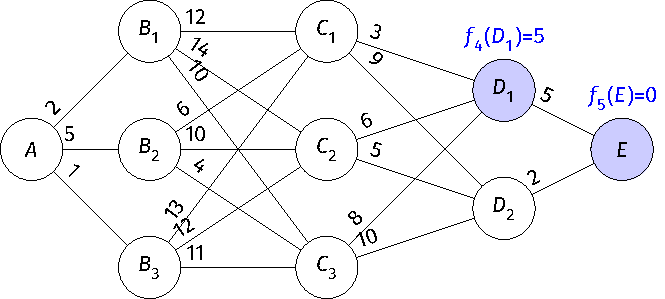
\includegraphics{fig/4-2-2.pdf}
    $$f_4(D_1)=d(D_1\rightarrow E)+f_5(E)=5+0=5$$
	\center{最优决策:$D_1\rightarrow E$ }
\end{frame}
\begin{frame}
    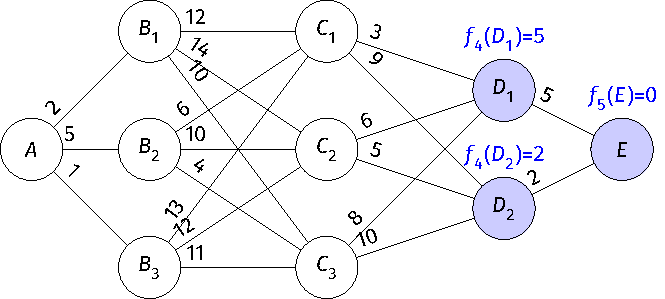
\includegraphics{fig/4-2-3.pdf}
    $$f_4(D_2)=d(D_2\rightarrow E)+f_5(E)=2+0=5$$
	\center{最优决策:$D_2\rightarrow E$ }
\end{frame}
\begin{frame}
    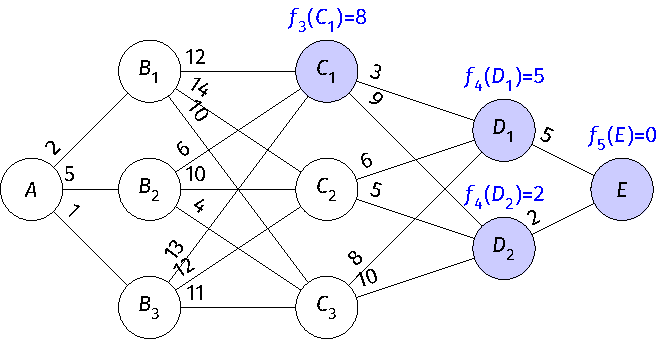
\includegraphics{fig/4-2-4.pdf}
    $$f_3(C_1)=min \begin{Bmatrix}(C_1,D_1)+f_4(D_1)\\\ (C_1,D_2)+f_4(D_2) \end{Bmatrix} =min \begin{Bmatrix}3+5\\\ 9+2 \end{Bmatrix} =8$$
	\center{最优决策:$C_1\rightarrow D_1$}
\end{frame}
\begin{frame}
    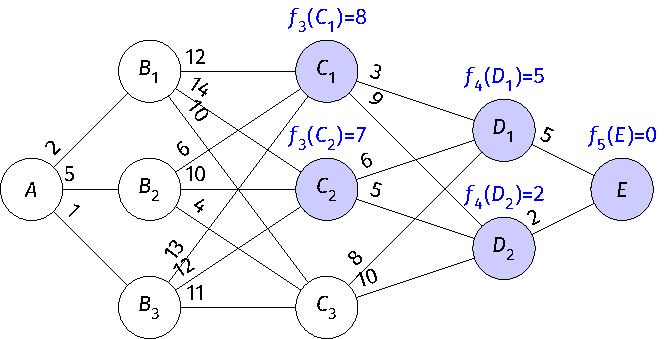
\includegraphics{fig/4-2-5.pdf}
    $$f_3(C_2)=min \begin{Bmatrix}(C_2,D_1)+f_4(D_1)\\\ (C_2,D_2)+f_4(D_2) \end{Bmatrix} =min \begin{Bmatrix}6+5\\\ 5+2 \end{Bmatrix} =7$$
	\center{最优决策:$C_2\rightarrow D_2$}
\end{frame}
\begin{frame}
    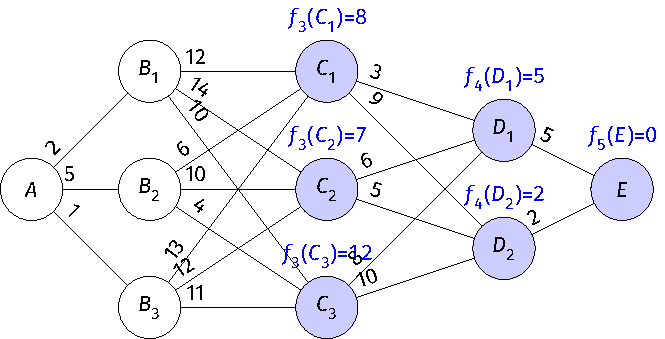
\includegraphics{fig/4-2-6.pdf}
    $$f_3(C_3)=min \begin{Bmatrix}(C_3,D_1)+f_4(D_1)\\\ (C_3,D_2)+f_4(D_2) \end{Bmatrix} =min \begin{Bmatrix}8+5\\\ 10+2 \end{Bmatrix} =12$$
	\center{最优决策:$C_3\rightarrow D_2$}
\end{frame}
\begin{frame}
    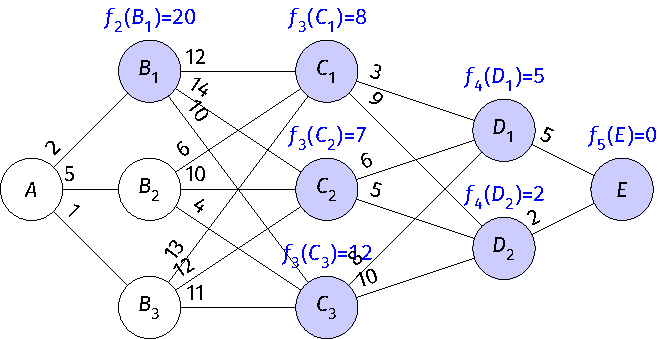
\includegraphics{fig/4-2-7.pdf}
    $$f_2(B_1)=min \begin{Bmatrix}(B_1,C_1)+f_3(C_1)\\\ (B_1,C_2)+f_3(C_2)\\\ (B_1,C_3)+f_3(C_3) \end{Bmatrix} =min \begin{Bmatrix}12+8\\\ 14+7\\\ 10+12 \end{Bmatrix} =20$$
	\center{最优决策:$B_1\rightarrow C_1$}
\end{frame}
\begin{frame}
    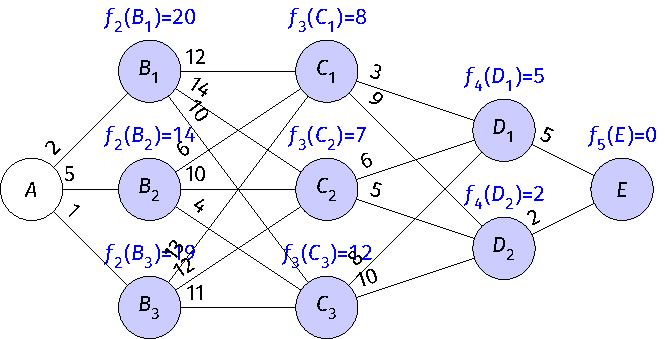
\includegraphics{fig/4-2-8.pdf}
    $$f_2(B_3)=min \begin{Bmatrix}(B_3,C_1)+f_3(C_1)\\\ (B_3,C_2)+f_3(C_2)\\\ (B_3,C_3)+f_3(C_3) \end{Bmatrix} =min \begin{Bmatrix}13+8\\\ 12+7\\\ 11+12 \end{Bmatrix} =19$$
	\center{最优决策:$B_3\rightarrow C_2$}
\end{frame}
\begin{frame}
    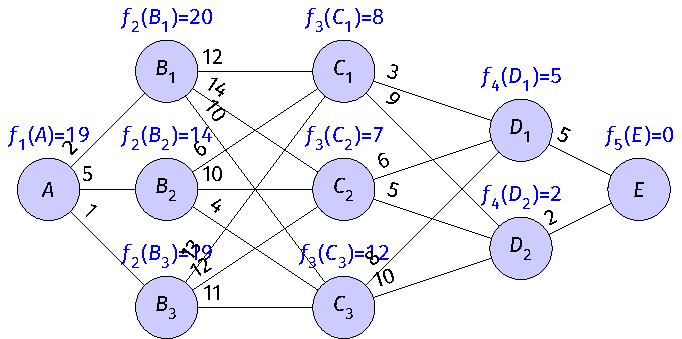
\includegraphics{fig/4-2-9.pdf}
    $$f_1(A)=min \begin{Bmatrix}(A,B_1)+f_2(B_1)\\\ (A,B_2)+f_2(B_2)\\\ (A,B_3)+f_2(B_3) \end{Bmatrix} =min \begin{Bmatrix}2+21\\\ 5+14\\\ 1+19 \end{Bmatrix} =19$$
	\center{最优决策:$A\rightarrow B_2$}
\end{frame}
\begin{frame}
    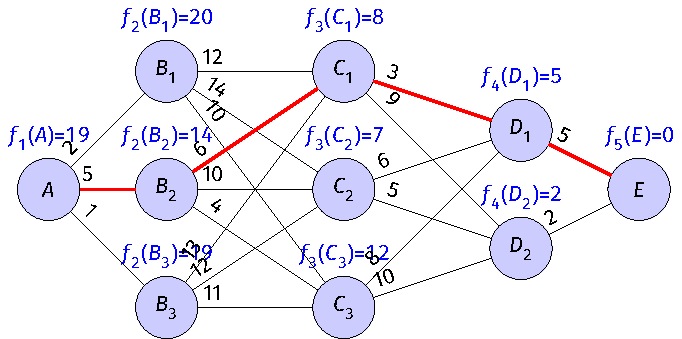
\includegraphics{fig/4-2-10.pdf}
    $$A\rightarrow B_2\rightarrow C_1 \rightarrow D_1 \rightarrow E$$
	\center{为$A$到$E$的最短路径,长度19}
\end{frame}
\begin{frame}{1163 -- The Triangle (poj.org)}
    \begin{itemize}
        \item 如图的数字三角形,从顶部出发,每一个结点可以选择向左或向右走,要求找到一个从上到下的路径,路径上数字的和最大
    \end{itemize}
    \vfill
    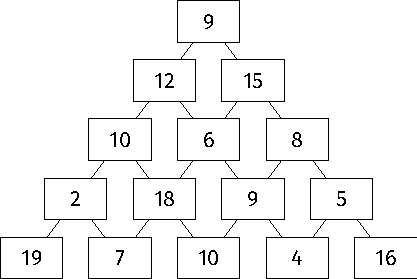
\includegraphics[center]{fig/4-3.pdf}
\end{frame}
\begin{frame}{1651 -- Multiplication Puzzle (poj.org)}
    \begin{itemize}
        \item n个数排成一排,从中间位置取走一个数,和它前后两个数相乘得到一个乘积值,再取一个数,继续计算, 直到剩下的最后三个数相乘,将所有乘积相加,求这个和的最小值
    \end{itemize}
    \vfill
    \begin{exampleblock}{Example: 10 1 50 20 5}
        \begin{itemize}
            \item 依次取1,20,50:
            $$10\times 1\times 50+50\times 20\times 5+10\times 50\times 5=500+5000+2500=8000$$
            \item 依次取50,20,1:
            $$1\times 50\times 20+1\times 20\times 5+10\times 1\times 5=1000+100+50=1150$$
        \end{itemize}
    \end{exampleblock}
\end{frame}
\begin{frame}{分析}
    \begin{itemize}
        \item \textcolor{blue}{区间动态规划}方法
        \begin{enumerate}[(1)]
            \item 定义二维数组D[i,j],i,j为区间左右两个边界
            \item 子区间的长度逐渐递增,直到原问题的区间长度为止
            \item 将子区间内的各种情况进行计算,保存最优值
            \item 由子问题的值推导上一层问题的值,直到计算结束
        \end{enumerate}
        \vfill
        \item 用a[1...n]保存n个数,D[i,j]为i到j区间计算出来的和的最小值,区间长度s=j-i,在区间内取一个位置k,则D[i,j]为所有D[i,k]+D[k,j]+a[i]\times a[k]\times a[j]的最小值
    \end{itemize}
\end{frame}
\begin{frame}{4.2 子序列问题}
    \begin{itemize}
        \item \textcolor{blue}{最长递增子序列}(Longest Increasing Subsequence, LIS)
        \vfill
        \begin{enumerate}
            \item 动态规划解法,复杂度为$O(n^2)$
            \begin{itemize}
                \item 用数组$D[i]$储存到$a[i]$为止包含$a[i]$的最长递增子序列的长度
                \item $D[i]=max⁡(D[j])+1,1\leq j < i$且$a[j] < a[i]$
            \end{itemize}
            \vfill
            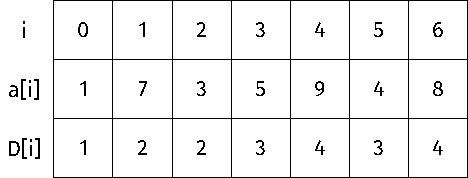
\includegraphics{fig/4-4.pdf}
            \vfill
            \item 二分查找 ,复杂度为$O(nlogn)$
        \end{enumerate}
    \end{itemize}
\end{frame}
\begin{frame}{2533 -- Longest Ordered Subsequence (poj.org)}
    \begin{itemize}
        \item A numeric sequence of $a_i$ is ordered if $a_1 < a_2 < ... < a_N$. Let the subsequence of the given numeric sequence $(a_1, a_2, ..., a_N)$ be any sequence $(a_{i_1}, a_{i_2}, ..., a_{i_K})$, where $1 \leq i_1 < i_2 < ... < i_K \leq N$.
        \item For example, sequence (1, 7, 3, 5, 9, 4, 8) has ordered subsequences, e. g., (1, 7), (3, 4, 8) and many others. All longest ordered subsequences are of length 4, e. g., (1, 3, 5, 8).
        \item Your program, when given the numeric sequence, must find the length of its longest ordered subsequence.
    \end{itemize}
\end{frame}
\begin{frame}{4.3 最长公共子串问题}
    \begin{block}{最长公共子序列}
        \textcolor{blue}{最长公共子序列} (Longest Common Subsequence, LCS) 是在一个序列集合中(通常为两个序列)查找所有序列中最长子序列的问题\\
        两个序列通常为两个字符串,此类问题也称为求\textcolor{blue}{最长公共子串}问题
    \end{block}
    \begin{itemize}
        \item $c[i,j]$表示从序列起点到 $x[i]$和$y[j]$时最长子序列的长度,则
    \end{itemize}
    $$c[i,j]=\begin{cases} c[i-1,j-1]+1, &x[i]=y[j] \\\ max(c[i-1,j],c[i,j-1]), &others \end{cases}$$
    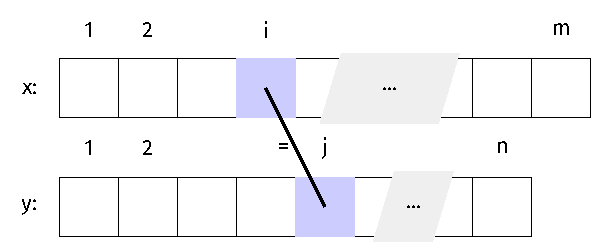
\includegraphics[scale=.7,center]{fig/4-5.pdf}
\end{frame}
\begin{frame}{1458 -- Common Subsequence (poj.org)}
    \begin{itemize}
        \item A subsequence of a given sequence is the given sequence with some elements (possible none) left out.
        \item Given a sequence $X=<x_1, x_2, ..., x_m>$ another sequence $Z=< z_1, z_2, ..., z_k>$ is a subsequence of $X$ if there exists a strictly increasing sequence $<i_1, i_2, ..., i_k>$ of indices of $X$ such that for all $j=1,2,...,k, x_{i_j}=z_j$
        \item For example, $Z=<a, b, f, c>$ is a subsequence of $X=<a, b, c, f, b, c>$ with	index sequence $<1, 2, 4, 6>$
        \item Given two sequences $X$ and $Y$ the problem is to find the length of the maximum-length common subsequence of $X$ and $Y$
    \end{itemize}
\end{frame}
\begin{frame}{4.4 背包问题}
    \begin{block}{背包问题}
        一组物品具有重量和价格,在规定的总重量内,如何选择,使得价格最高,被称为\textcolor{blue}{背包问题}\footnote{\url{https://github.com/tianyicui/pack}}(Knapsack problem)
    \end{block}
    \begin{itemize}
        \item \textcolor{blue}{0-1背包问题}: 每种物品仅有一件,可以选择放或不放
        \begin{itemize}
            \item 用动态规划来求解背包问题,通过子问题定义状态:即$F[i,v]$表示前$i$件物品恰放入一个容量为$v$的背包可以获得的最大价值,
            则当前最优解要么包含第$i$种物品,要么不包含第$i$种物品,状态转移方程:
            $$F[i,v]=\max\begin{cases} F[i-1,v] \\\ F[i-1,v-c[i]+w[i]] \end{cases} $$
            \item 时空复杂度均为$NV$,只用一维数组$F[j]$可以降低空间复杂度
            \item 恰好装满 $F[0]=0$,$F[1\ldots V]=-\infty$;不要求装满 $F[1\ldots V]=0$
        \end{itemize}
    \end{itemize}
\end{frame}
\begin{frame}{3624 -- Charm Bracelet (poj.org)}
    \begin{itemize}
        \item Bessie has gone to the mall's jewelry store and spies a charm bracelet. Of course, she'd like to fill it with the best charms possible from the $N(1\leq N\leq 3,402)$ available charms.
        \item Each charm $i$ in the supplied list has a weight $W_i(1\leq W_i\leq400)$, a 'desirability' factor $D_i(1\leq D_i\leq 100)$, and can be used at most once. Bessie can only support a charm bracelet whose weight is no more than $M(1\leq M\leq 12,880)$.
        \item Given that weight limit as a constraint and a list of the charms with their weights and desirability rating, deduce the maximum possible sum of ratings.
    \end{itemize}
\end{frame}
\begin{frame}{分析}
    \begin{itemize}
        \item $n$个物品,每个物品有$w$和$d$属性,要求选出一定的物品,在$\sum w$不超过$m$的情况下,使得$\sum d$最大
    \end{itemize}
    \vfill
    \begin{exampleblock}{Example}
        \begin{columns}
            \column{0.5\textwidth}
            \begin{table}
                \begin{tabular}{cc}
                4 & 6 \\\hline
                \alert{1} & \alert{4} \\\hline
                2 & 6 \\\hline
                \alert{3} & \alert{12} \\\hline
                \alert{2} & \alert{7} \\\hline
                \end{tabular}
            \end{table}
            \column{0.5\textwidth}
            \begin{table}
                \begin{tabular}{cc}
                $n$ & $m$ \\\hline
                $w_1$ & $d_1$ \\\hline
                $w_2$ & $d_2$ \\\hline
                $w_3$ & $d_3$ \\\hline
                $w_4$ & $d_4$ \\\hline
                \end{tabular}
            \end{table}
        \end{columns}
    \end{exampleblock}
\end{frame}    
\begin{frame}{完全背包问题}
    \begin{itemize}
        \item \textcolor{blue}{完全背包问题}: 有$n$种物品和一个容量为$V$的背包,每种物品都有无限件可用
        \vfill
        \item 在0-1背包基础上,将添加第$i$件物品的情况考虑到已经选择过第$i$件物品的情况
        \begin{itemize}                
            \item 0-1背包:$v=V\rightarrow 0$,保证每件物品选一次
            \item 完全背包:$v=0\rightarrow V$,每种物品可选无限件
        \end{itemize}
        \vfill
        \item 恰好装满$F[0]=0$,$F[1\ldots V]=-\infty$;不要求装满 $F[1\ldots V]=0$
    \end{itemize}
\end{frame}       
\begin{frame}{1384 -- Piggy-Bank (poj.org)}
    \begin{itemize}
        \item $n$种不同的硬币,有两个属性,$p$代表金额,$w$代表重量,钱罐空时重$e$,满时重$f$,计算满时钱罐里最小可能的总金额是多少
    \end{itemize}
    \vfill
    \begin{exampleblock}{Example}
        \begin{columns}
            \column{0.5\textwidth}
            \begin{table}
                \begin{tabular}{cc}
                10 & 110 \\\hline
                2 &  \\\hline
                1 & 1 \\\hline
                \alert{30} & \alert{50} \\\hline
                \end{tabular}
            \end{table}
            \column{0.5\textwidth}
            \begin{table}
                \begin{tabular}{cc}
                $e$ & $f$ \\\hline
                $n$ \\\hline
                $p_1$ & $w_1$ \\\hline
                $p_2$ & $w_2$ \\\hline
                \end{tabular}
            \end{table}
        \end{columns}
    \end{exampleblock}
\end{frame}  
\begin{frame}{多重背包问题}
    \begin{itemize}
        \item \textcolor{blue}{多重背包问题}: 一种物品有$m$个(既不是固定的1个,也不是无数个)
        \vfill
        \item 多重背包$c$为费用,$w$为价值,$m$为数量
        \begin{itemize}                
            \item 当$c\times m$超过$V$,直接采用完全背包
            \item 否则将$m$进行拆分,拆分成$$1,2,4,…,2^k-1,𝑚−(2^k-1)$$
            \item 然后进行0-1背包
        \end{itemize}
        \vfill
        \item 例如$m=13$,拆成$1,2,4,6$
    \end{itemize}
\end{frame}       
\begin{frame}{1276 -- Cash Machine (poj.org)}
    \begin{itemize}
        \item 有$N$台提款机,每台提款机提供不同数量$n_i$和面值$D_i$的货币,求这些机器能提取的不超过指定限额$cash$的最大金额
    \end{itemize}
    \vfill
    \begin{exampleblock}{Example}
        \begin{table}
            \begin{tabular}{cccccccccc}
                $cash$ & $N$    & $n_1$   & $D_1$   & $n_2$   & $D_2$   & $n_3$   & $D_3$   & $n_N$   & $D_N$  \\\hline
                735  & 3    & 4    & 125  & 6    & 5    & 3    & 350  &      &    \\\hline
                633  & 4    & 500  & 30   & 6    & 100  & 1    & 5    & 0    & 1  \\\hline
            \end{tabular}
        \end{table}
        \begin{table}
            \begin{tabular}{cccccccccc}
                 & $n_1$   & $D_1$   & $n_2$   & $D_2$   & $n_3$   & $D_3$   & $n_N$   & $D_N$  \\\hline
                735  & 3  & 125  & 2    & 5    & 1    & 350  &      &    \\\hline
                633  & 1  & 30   & 6    & 100  & 0    & 5    & 0    & 1  \\\hline
            \end{tabular}
        \end{table}  
    \end{exampleblock}
\end{frame}  
\end{document}